\chapter{Basic Programming of the QCDSP}
\section{Introduction}
This chapter is intended as a guide to the basic
system calls implemented on the QCDSP computer.

The QCDSP itself is most simply programmed in C or 
C++, for which a commercial compiler exists with
some optimisation features. The compiler is called
the Tartan C++ compiler and the UNIX invocation of it 
is via the command {\tt tcpp}. 

The machine can also be programmed at the assembler
level and  indeed such programming may be necessary to achieve
maximal computational and communication performance. However,
for the moment we shall not discuss this mode of programming. 

\section{Parallelism in the QCDSP Computer}
The QCDSP, whether at the level of a single development board
or at the level of several cabinets containing processor boards
is a MIMD\footnote{Multiple Instruction Multiple Data} parallel computer. 

This means, that each processor is capable of running completely
independent code. However, the machine is 
perhaps best programmed according to the SPMD\footnote{Single Program Multiple Data} programming model. In this programming model processors run the 
same program, using different datasets resident to each processor. Also
this programming model allows one to write fully MIMD programs, by executing
separate subroutines (of the same program) depending on some identification
token (a unique processor ID, processor grid coordinates or some such) 
from the local processor. 

Furthermore, the QCDSP has a distributed memory, with no current
implementation of a shared memory system. The preferred method of 
communication is via message passing between neighbouring processors.
We shall outline possible methods to implement global communications
such as broadcasts and global sums in the next chapter.
For the current chapter, we shall introduce some of the QCDSP system
calls to allow a given particular processor to identify itself, and 
to send messages to its neighbours. To make the discussion clearer,
we have to mention a few details about the architecture and network
topology of the QCDSP computer.

\section{Brief description of the QCDSP Architecture}
The QCDSP at the bottom level consists of a collection of Texas
Instruments TMS320C31 Digital Signal Processors (DSPs) with associated
DRAM memory (0.5Gwords of error correcting memory per processor) and
special purpose communications hardware. These components are
organised into a hierarchy of {\em daughterboards}, {\em motherboards}
and {\em crates}.

A daughterboard consists of a single DSP chip, its associated DRAM and 
its so called Node Gate Array (NGA), which is the communications unit
built on a custom chip. A single daughterboard is about the size of a 
credit card. A picture of a daughterboard is shown in figure \ref{f:daughterBoard}
\begin{figure}[ht]
\begin{center}
\leavevmode
\hbox{%
\includegraphics{daughterboard_photo}
}
\end{center}
\caption{Photograph of a daughterboard. The DSP chip and the NGA are shown
with a ruler to indicate size in inches}
\label{f:daughterBoard}
\end{figure}

The daughterboards are themselves mounted on motherboards. A single
motherboard holds up to 64 daughterboards. Of these, one daughterboard
(daughterboard 0) is integrated onto the motherboard and has some 
special functions that we shall describe later. A picture of a motherboard 
can be seen in figure \ref{f:motherBoard}.

\begin{figure}[ht]
\begin{center}
\leavevmode
\hbox{%
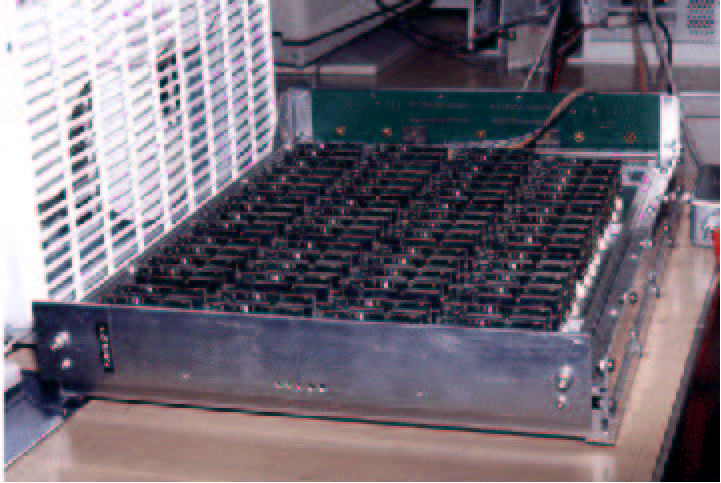
\includegraphics[width=4in]{motherboard_photo}
}
\end{center}
\caption{Photograph of a motherboard containing 63 daughterboard cards and
one integrated daughterboard. The motherboard is mounted on a test rig and 
is cooled by the fan on the left hand side}
\label{f:motherBoard}
\end{figure}

The daughterboards are connected on the motherboard in a four dimensional 
(4D) mesh via a {\em serial network} which is intended to be the main 
medium of communications for applications and hence it has been named
{\em the physics network}. The physics network is driven by the NGA 
of each daughterboard. This 4D serial network wraps around in each dimension,
giving each motherboard network topology of a {\em 4D--torus}.

All the daughterboards on a given motherboard are also connected to the 
special daughterboard 0 (the one integrated on the motherboard) via
a second serial network in a star topology. This network is part
of the so called {\em boot--diagnostic network}. The boot--diagnostic
network is used for hardware testing, and for downloading the various
boot and runtime kernels to the daughterboards at boot time. 

Each motherboard also has two SCSI ports which are connected to
daughterboard 0 on that board. These ports allow the connection of
daughterboards to either a front end host, to another motherboard, or
in future designs of the machine, to local disk systems. The SCSI
connections form part of the boot--diagnostic network and are not in
general expected to be heavily used in physics applications.

The motherboards are organised into crates. The {\em physics networks}
of the boards in a given cabinet are connected by a tagliatelle tangle
of flat ribbon serial cables into an overall physics network which
still forms a 4D torus.  The boot diagnostic networks of the boards in
a crate are connected via the SCSI interfaces on the motherboards into
a tree hierarchy. A picture of a crate is shown in figure \ref{f:crate}.
\begin{figure}[ht]
\begin{center}
\leavevmode
\hbox{%
\includegraphics{crate_photo}
}
\end{center}
\caption{A QCDSP crate holding 6 motherboards}
\label{f:crate}
\end{figure}

Finally the crates are assembled into a full machine.

In summary the communications in a machine are made up of two networks:
\begin{itemize}
\item
The Physics Network -- which is a serial network that to the programmers
point of view forms a 4D torus. This is the network that is intended for 
primary communications in an application.
\item
The Boot--Diagnostic network made up from a SCSI chain between motherboards,
rooted on the front end workstation. On each motherboard the boot--diagnostic
network is constructed from a serial network with a star topology rooted
on daughterboard 0.
\end{itemize}

A summary of the networks in QCDSP can be seen in figure \ref{f:networkSummary}.
\begin{figure}[ht]
\begin{center}
\leavevmode
\hbox{%
\includegraphics[width=4in]{networks_summary}
}
\end{center}
\caption{A summary diagram of QCDSP Networks showing three motherboards
connected in a tree of depth = 2. The horizontal and vertical
black lines show the physics network (2 dimensions of it) with the black
dots showing the daughterboards. The green lines show the SCSI tree and 
the red lines show the serial boot--diagnostic network. Purple lines 
show the connections between the SCSI ports and motherboard 0 on each 
board.}
\label{f:networkSummary}
\end{figure}

\section{Programming Interface}
The QCDSP at the simplest level provides a set of C++ functions
which may be called to achieve various aims. Broadly these functions
can be categorised as
\begin{itemize}
\item
Functions allowing the processor to identify itself and the machine
\item
Objects and functions for carrying out communications
\item
functions for self synchronisation
\item
miscellany -- random numbers etc .
\end{itemize}

\subsection{Header Files}
These functions are defined in the header file {\bf sysfunc.h} in the
directory {\tt /qcdsp/sfw/qos.<version>/usr/include} where {\tt
<version>} refers to the QOS revision as discussed in the previous
chapter. This directory should be listed as part of the {\tt TC\_DIR}
shell environment variable (see last chapter), thus making the
directory part of the default search path for the Tartan C++
compiler. The programmer merely needs to include the header file in
his source files using the directive
\begin{verbatim}
#include <sysfunc.h>
\end{verbatim} 
identically to the way he/she normally includes {\bf stdio.h}, {\bf stdlib.h}, 
{\bf math.h} and other standard header files.

\subsection{Unsupported C++ Features}
One should also be aware that not all of the standard ANSI C++ libraries
are implemented on the QCDSP. In particular the {\tt iostream} classes
are unavailable. The programmer needs to use the C standard I/O routines
defined in {\bf stdio.h}.

\subsection{Compilation and Running of Examples}
In the following sections we describe some of the functions provided 
in the {\bf sysfunc.h} file. To run the example codes we recommend that
the reader copies the {\em hello\_world} program as described in the last
section into his homedirectory and modifies the file {\bf main.C}. The makefile
provided can then be used to build the examples by typing the command {\tt make}. The resulting executable will be called {\bf hello\_world.out}. (Readers
with a knowledge of makefiles can adapt the makefile as they wish. The compiler
flags and command line options for the C++ compiler can be listed by typing
the command {\tt tcpp} with no arguments.) Let us
assume from here on that the {\em hello\_world} directory was copied to one
of identical name in the users homedirectory and that the results of all
compilations are named {\bf hello\_world.out}.

\section{Who Am I?}
\subsection{Knowing your identity and place in the Universe}
The following functions are defined in {\bf sysfunc.h} to enable
a processor to localise itself:
\begin{description}
\item{\tt int UniqueID()\ : \\}
This function returns an {\tt int} specifying 
the {\bf unique processor ID} of the calling
processor. (N.B: The MPI equivalent of this call
would be {\tt MPI\_Comm\_Rank}).
\item{\tt int NumNodes()\ : \\}
This function returns an {\tt int} specifying 
the total number of nodes
that are in use in the current machine partition.
(N.B: The MPI equivalent of this call would be {\tt MPI\_Comm\_Size}).
\item{\tt int MbNum()\ : \\}
This function returns an {\tt int} specifying the {\bf motherboard number}
of the motherboard on which the calling processor resides.
\item{\tt int DbNum()\ : \\}
This function returns an {\tt int} specifying the {\bf daughterboard number}
of the calling processor.
\item{{\tt int CoorT()}, {\tt int CoorX()}, {\tt int CoorY()}, {\tt int CoorZ()} \ : \\}
These function calls return {\tt int}-s specifying the T, X, Y and Z coordinates respectively, of the calling processor within the 4D torus of the physical
network.
\item{{\tt int SizeT()}, {\tt int SizeX()}, {\tt int SizeY()}, {\tt int SizeZ()} \ : \\} 
These functions return {\tt int}-s specifying the size of the 4D torus physical
network in the T, X, Y and Z directions respectively
\end{description}

Figure \ref{f:whoamiCode} shows a programming example, where the processors
in the QCDSP identify themselves and size up their machine parition using
these functions:
\begin{figure}[h]
\tiny
\begin{verbatim}
#include <stdio.h>
#include <stdlib.h>
#include <sysfunc,h>

int main(int argc, char *argv[])
{
   /* ------- What is my Unique ID  ---------------------- */
   int my_id = UniqueID();
   int num_processors = NumNodes();

   /* ------- Motherboard and Daughterboard Numbers -------*/
   int my_motherboard_num = MbNum();
   int my_daughterboard_num = DbNum();

   /* - My processor grid coordinates and grid dimensions -*/
   int my_coords[4];
   int proc_grid_dims[4];

   /* --------------- Get my coordinates ----------------- */
   my_coords[0] = CoorT();
   my_coords[1] = CoorX();
   my_coords[2] = CoorY();
   my_coords[3] = CoorZ();

   /* - Get information about the processor grid size ---  */
   proc_grid_dims[0] = SizeT();
   proc_grid_dims[1] = SizeX();
   proc_grid_dims[2] = SizeY();
   proc_grid_dims[3] = SizeZ();

   /* -  Echo Back information to the user --------------- */
   printf("I am processor: %d.\n", my_id);
   printf("I live on motherboard %d, daughterboard %d\n",  my_motherboard_num,
                                                             my_daughterboard_num);

   printf("I am one of a total of %d computing elements\n", num_processors);
  
   printf("The current physical network has the following dimensions\n");
   printf("%d Processors in the T direction\n", proc_grid_dims[0]);
   printf("%d Processors in the X direction\n", proc_grid_dims[1]);
   printf("%d Processors in the Y direction\n", proc_grid_dims[2]);
   printf("%d Processorz in the Z direction\n", proc_grid_dims[3]);
  
   printf("My (T,X,Y,Z) coordinates are (%d, %d, %d, %d )\n", 
           my_coords[0], my_coords[1], my_coords[2], my_coords[3]);

   return(EXIT_SUCCESS);
}
\end{verbatim}
\caption{Sample program showing use of self identification functions.}
\label{f:whoamiCode}
\end{figure}   

Running the code in figure \ref{f:whoamiCode} on the 64 daughterboard 
development board {\em q\_2} produced the following results:
{
\scriptsize
\begin{verbatim}
(qcdhost/homeqs0/bj/hello_world: qcsh[q_2])% qrun hello_world.out
.
.
.
I am processor: 0.
I live on motherboard 0, daughterboard 0
I am one of a total of 64 computing elements
The current physical network has the following dimensions
4 Processors in the T direction
4 Processors in the X direction
2 Processors in the Y direction
2 Processorz in the Z direction
My (T,X,Y,Z) coordinates are (0, 0, 0, 0 )
.
.
.
\end{verbatim}
}

Using the command {\tt qprintf} command as described in the last chapter
allows one to look at the output buffers of some of the other processors:
{\scriptsize
\begin{verbatim}
.
.
.
Qdaemon:  user print buffer for Mb 0 and Db 2 (SCSI tree coordinates)
Buffer wrap count 0
I am processor: 2.
I live on motherboard 0, daughterboard 2
I am one of a total of 64 computing elements
The current physical network has the following dimensions
4 Processors in the T direction
4 Processors in the X direction
2 Processors in the Y direction
2 Processorz in the Z direction
My (T,X,Y,Z) coordinates are (0, 0, 1, 0 )
.
.
.
Qdaemon:  user print buffer for Mb 0 and Db 63 (SCSI tree coordinates)
Buffer wrap count 0
I am processor: 63.
I live on motherboard 0, daughterboard 63
I am one of a total of 64 computing elements
The current physical network has the following dimensions
4 Processors in the T direction
4 Processors in the X direction
2 Processors in the Y direction
2 Processorz in the Z direction
My (T,X,Y,Z) coordinates are (3, 3, 1, 1 )
\end{verbatim}
}

\subsection{Some useful enumerated types}
You may notice\footnote{if you haven't yet please do so now}
if you look through the code in \ref{f:whoamiCode} that
I have always ordered the indices of both the {\tt my\_coords} and {\tt proc\_grid\_dims} in the order T, X, Y and Z with the T corresponding to the index
0 and Z corresponding to index 3. To make for much more
readable programs there exists an enumerated type called {\tt SCUAxis}.
A variable of type {\tt SCUAxis} can take on only four values
\begin{description}
\item{\tt SCU\_T -- \ } 
for the T direction,
\item{\tt SCU\_X -- \ } 
for the X direction,
\item{\tt SCU\_Y -- \ } 
for the Y direction and 
\item{\tt SCU\_Z -- \ } 
for the Z direction \ .
\end{description}
The actual definition of the type:
{\scriptsize \begin{verbatim}
enum SCUAxis { SCU_T, SCU_X, SCU_Y, SCU_Z };
\end{verbatim}}
ensures that the integer values of the enumerations
are {\tt SCU\_T}=0, {\tt SCU\_X}=1, {\tt SCU\_Y}=2 and {\tt SCU\_Z}=3
respectively. 

Thus we should be able to index our arrays with these enumerations
rather than with the integers 0,1,2 and 3 as before. For example
we could write
{\scriptsize \begin{verbatim}
my_coords[SCU_X]=CoorX(); /* equivalent to my_coords[1] = CoorX() */
\end{verbatim}} 
or for example we could cycle through all the directions in the 
processor grid with the following {\tt for} loop:
{\scriptsize \begin{verbatim}
int i;
for(i = SCU_T; i <= SCU_Z; i++) {
  /* do something exciting here  */
}
\end{verbatim}}

Incidentally, we note that this latter use relies on the particular
ordering of the axes defined in the enumerated type. In future releases
of QOS, the ordering of the enumerated elements maybe different from 
the current release. If this happens the above for loop may not be 
portable. Hence, {\em caveat emptor}. The enumerated type itself 
is defined in {\tt /qcdsp/sfw/qos.<version>/include/scu\_enum.h} which
is included in the {\bf sysfunc.h} file. ({\em Suggestion:
perhaps a member of the enumerated type called MAX\_AXIS or something
should be defined for such loops. They could then be written as
} {\tt for(i=0; i< MAX\_AXIS; i++) })

\section{Nearest Neighbour Communications}
The QCDSP {\bf sysfunc.h} header files defines several ways of carrying
out nearest neighbour communications. We will look into the simplest one
here. By communication we mean sending/receiving a certain number of bytes
from one processor to another. On the QCDSP such a communication is made up of
three stages.
\begin{description}
\item{\bf Preparation: \ } -- the sender/receiver describes the data
to be sent/received and provides a pointer in memory to the data that
is to be sent / to where the data is to be received
\item{\bf Initiation: \ } --  the sender / receiver initiates the 
communication. The sender / receiver is then free to carry out other
tasks.
\item{\bf Completion: \ } -- the sender / receiver wait until the 
communication is complete, in the case of the sender this means that 
all the data has been sent and in the case of the receiver it means that
the the data has arrived.
\end{description}
Communication along the physical network is handled by the Serial
Communication Unit (SCU) in the NGA chip, and the communication does
not need much interaction from the CPU past the initiation
stage. Hence the time spent communicating allows the processor to
carry out computation while the communication proceeds. It is only
immediately before using the results of the communications that the
processor has to wait to make sure that the communication is
complete. (Note: This is similar in style to the MPI non--blocking
communications, however in the case of MPI the so called preparation
and initiation stages are usually rolled into one)

\subsection{Preparation}
In preparing to communicate we must decide upon the following things:
\begin{itemize}
\item
Who did we want to communicate with? This is generally one of our
neighbours. We have neighbours in eight directions, these being 
the positive and negative T, X, Y and Z directions respectively. An enumerated type, {\tt SCUDir}, is made available to help us in writing safe, 
maintainable programs. This enumerated type is made accessible through
the header file {\bf sysfunc.h}. The actual enumerations are
\begin{description}
\item{ {\tt SCU\_TM} (T, Minus): \ } 
-- Communicate in the negative T direction
\item{ {\tt SCU\_TP} (T, Plus): \ } 
-- Communicate in the positive T direction
\item{ {\tt SCU\_XM} (X, Minus): \ }
-- Communicate in the negative X direction
\item{ {\tt SCU\_XP} (X, Plus) : \ }
-- Communicate in the positive X direction
\item{ {\tt SCU\_YM} (Y, Minus): \ } 
-- Communicate in the negative Y direction
\item{ {\tt SCU\_YP} (Y, Plus): \ } 
-- Communicate in the positive Y direction
\item{ {\tt SCU\_ZM} (Z, Minus): \ }
-- Communicate in the negative Z direction
\item{ {\tt SCU\_ZP} (Z, Plus) : \ }
-- Communicate in the positive Z direction
\end{description}
\item 
We must decide whether we wish to send a message or receive one.
Once again we have an enumerated type at our disposal called
{\tt SCUXR}. This can have only two values:
\begin{description}
\item{ {\tt SCU\_REC} : \ } 
receive operation
\item{ {\tt SCU\_SEND} : \ } 
send operation.
\end{description}
\item
We must describe our data. For our purposes the data shall consist 
of a number of blocks, each block having a certain length. The blocks
need not be contiguous in memory, but may have some regular spacing
between them. The distance in memory ({\bf in units of blocks}) separating
the {\bf start of one block} from the {\bf start of the next one} is called
the data stride.

Hence our messages are completely described by specifying the {\em
memory address} of the first block, {\em the length of a block in
bytes}, {\em the number of blocks in the message} and {\em the
stride}.  For messages made up of a contiguous set of blocks, the
stride is always one. In other words, the start of a block in memory is
always one block-length away from the start of the previous block with the
intervening memory between the two being filled up by the body of
the first block. The idea of this data description scheme is illustrated
in figure \ref{f:message}.
\end{itemize}

\begin{figure}[h]
\begin{center}
\leavevmode
\hbox{
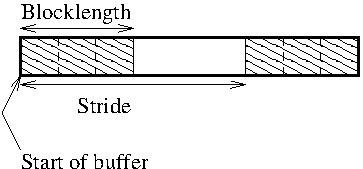
\includegraphics{message}}
\end{center}
\caption{Anatomy of a message. Here the message consists of 2 blocks
(shaded) with each block having a block length of 3 bytes. The blocks
are not contiguous but have a block separation between them making the
stride value for this message 2}
\label{f:message}
\end{figure}

On the QCDSP the preparing to communicate involves the instantiation
of a so called {\tt SCUDirArg} object. There are several ways of
carrying out this instantiation. Perhaps the simplest is to use the
{\em constructor}: 
{\small \begin{verbatim} 
SCUDirArg(void *buffer, SCUDir dir, SCUXR xr, int blklen, 
          int numblk = 1, int stride = 1).
\end{verbatim}}
This method allows the complete description of the putative communication to be specified with one single statement. The arguments have the following meaning:
\begin{description}
\item{\tt void *buffer \ } 
this is a pointer to the start of the message in memory. It is of type {\tt void *} so that the pointer can point to data of any type. 
\item{\tt SCUDir dir \ } 
this is the direction in which the communication is to proceed and should take
the value of one of the 8 enumerations of the enumerated type {\tt SCUDir } listed above.
\item{\tt SCUXR xr \ } 
indicates whether we are sending or receiving. This should take one of the two 
values of the enumerated type {\tt SCUXR} listed above.
\item{\tt int blklen \ } 
gives the length in bytes of a single block to be transmitted/received.
\item{\tt int numblk = 1 \ }
gives the number of blocks to be communicated. This is an optional
argument to the constructor, which, if unspecified will have the
default value of 1, indicating that there is only a single block to be
communicated
\item{\tt int stride = 1 \ }
specifies the stride of the data. This is an optional argument to the constructor, which, if unspecified will have the default value of 1 corresponding to the 
contiguous data.
\end{description}

As an example, suppose I wanted to send an integer in the 
positive X direction, I could instantiate the communication description object as:
\begin{verbatim}
int number_to_send = 5;
SCUDirArg send_int_x_plus((void *)&number_to_send, SCU_XP, 
                          SCU_SEND, sizeof(int));
\end{verbatim}
or as:
\begin{verbatim}
int number_to_send = 5;
SCUDirArg send_int_x_plus((void *)&number_to_send, SCU_XP, 
                                  SCU_SEND, sizeof(int),1);
\end{verbatim}
or even as:
\begin{verbatim}
int number_to_send = 5;
SCUDirArg send_int_x_plus((void *)&number_to_send, SCU_XP, 
                                  SCU_SEND, sizeof(int),1,1);
\end{verbatim}
where in the last two cases I have explicitly specified the optional arguments.
In all the above cases the result of the instantiation is an
object of type {\tt SCUDirArg} with name {\tt send\_int\_x\_plus}. This object
now acts as a {\em handle} to that particular communication.

Likewise to receive a 5-vector of floating point numbers of type {\tt float}
from the negative Y direction, I would set up the communication as:
\begin{verbatim}
float receive_buffer[5];
SCUDirArg rec_floats_y_minus((void *)receive_buffer, SCU_YM, 
                             SCU_REC, sizeof(float), 5, 1);
\end{verbatim}

Alternatively, I can set up the communication to send the 5 members of a 10 member integer array which have odd indices in the positive T direction using the
following instantiation:
\begin{verbatim}
int send_buffer[10];
SCUDirArg send_odd_t_plus((void *)&send_buffer[1], SCU_TP, 
                          SCU_SEND, sizeof(int), 5, 2);
\end{verbatim}

The {\tt SCUDirArg} objects can also be instantiated and manipulated using
various other {\em class methods}. For example I can instantiate an
object, without a description of the communication to be performed 
by simply using the default constructor:
\begin{verbatim}
SCUDirArg for_later;
\end{verbatim}
Later on I can initialise this object with the method {\tt Init}
which has the same argument list as the full constructor described earlier.
Hence I can either set up the object in the previous manner as:
\begin{verbatim}
int number_to_send = 5;
SCUDirArg send_int_x_plus((void *)&number_to_send, SCU_XP, 
                          SCU_SEND, sizeof(int));
\end{verbatim}
or alternatively I can use the {\tt Init} method:
\begin{verbatim}
int number_to_send = 5;
SCUDirArg send_int_x_plus;
send_int_x_plus.Init((void *)&number_to_send, SCU_XP, 
                          SCU_SEND, sizeof(int));
\end{verbatim}

Other methods by which the data description elements of the object can be
set are
\begin{description}
\item{\tt void * Addr( void *addr) \ }
the start of the data is set to {\tt addr}. The address of the new
buffer is returned.
\item{\tt int Blklen( int blklen ) \ }
the block length of the communication is set to {\tt blklen}. The 
new block length is returned.
\item{\tt int Numblk( int numblk ) \ }
the number of blocks in the transfer is set to {\tt numblk}. The new
number of blocks is returned.
\item{\tt int Stride( int stride ) \ } 
the stride of the transfer is set to {\tt stride}. The new stride is returned.
\item{\tt void Reload(void *a, int blklen, int numblk=1, int stride = 1) \ }
The new data description indicated in the argument list is set (the send/receive nature of the data or the communication direction remain as before). {\tt a} holds the address of the start of the data. The remaining arguments should be
self explanatory by now. Note again that the last two arguments are optional.
\end{description}

So for example to send first an {\tt int}, then a {\tt float} in the 
positive X direction followed by a second {\tt int} communication, I can 
instantiate the communication object for the first {\tt int}  and then simply
use the methods above to change the data description:
\begin{verbatim}
int int_buf=5;
int float_buf=0.6;

/* Set up the integer communications */

SCUDirArg send_x_plus((void *)&int_buf, SCU_XP, 
                      SCU_SEND, sizeof(int));

/* 
 * Carry out the first communications here 
 */

/* Now change to float communications -- send in the same direction */
send_x_plus.Addr((void *)&float_buf);
send_x_plus.Blklen(sizeof(float));
 
/* 
 * Carry out the second communication here
 */

/* Now prepare to send  an int again -- last two arguments optional */
send_x_plus.Reload((void *)&int_buf, sizeof(int));

/*
 * Carry out the third communication here
 */
\end{verbatim}

\subsection{Initiating the Communications}
Once we have defined the type of communication we wish to perform,
we must initiate the data transfer. This is done by the function
{\tt SCUTrans}. There are several ways of using {\tt SCUTrans}, here I will
describe the simplest one.

Calling {\tt SCUTrans} with the address of an {\tt SCUDirArg} object as the 
sole argument will initiate the communication encoded in that object.

As an example, suppose we want to send the integer 4 in the positive X
direction and an {\tt SCUDirArg} object {\tt int\_x\_plus} has been
instantiated to describe this communication ({\em Exercise:
Instantiate an SCUDirArg object to encode this communication.}) The
communication could then be initiated by the following call:
\begin{verbatim}
SCUTrans( &int_x_plus );
\end{verbatim}
However the results of the communication will not be available until the
communication completes.

\subsection{Completing the Communication}
To complete the communication the program should call the function
{\tt SCUTransComplete}. One can call this function with the address
of an {\tt SCUDirArg} object to complete to communication encoded in 
that, or without any arguments to complete all outstanding communications.
There is also another way to call {\tt SCUTransComplete} to match a 
particular way of calling {\tt SCUTrans} which will not be detailed here.

Hence to complete the previously initiated transfer encoded in the object
{\tt x\_int\_plus} of the last subsection, one should call
\begin{verbatim}
SCUTransComplete( &x_int_plus);
\end{verbatim}

To complete all outstanding communications on a given processor ({\bf
this does not imply a synchronisation across processors}) one should
instead call 
\begin{verbatim}
SCUTransComplete();
\end{verbatim}

\section{Getting To Know Your Neighbours}
Before concluding this chapter, we present the code for a complete program
designed to show the use of some of the communication routines presented
in the last section. 

The program discovers the processor ID's of its neighbours in every direction.
For each axis, T, X, Y and Z, the processors send their unique ID's in the
positive direction, and receive the ID's of their neighbours from the negative
direction.

Once this is done for all four axes, the communication pattern is
repeated but in the opposite direction. That is, for all four axes,
each processor will send its unique ID in the negative direction and
receives the ID of its neighbour from the positive direction.  When
this process is done for all the axes, the processor will have the ID's of
all its neighbours.

{\scriptsize
\begin{verbatim}
#include <stdio.h>
#include <stdlib.h>
#include <sysfunc.h>

// --------------------------------------------------------------------
// This function, when given the direction to send in (send direction)
// will send the contents of its send_buffer in that direction and 
// will receive into its receive buffer from the negative direction
// -------------------------------------------------------------------
void neighbourSend(int *send_buffer, int *recv_buffer,
                   SCUDir send_direction)
{

   SCUDir recv_direction;

   // ------------------------------------------------------------- //
   // Figure out the receive direction                              //
   // ------------------------------------------------------------- //

   switch( send_direction ) {

        case SCU_TM : recv_direction = SCU_TP;
                        break;

        case SCU_TP : recv_direction = SCU_TM;
                        break;

        case SCU_XM : recv_direction = SCU_XP;

                      break;

        case SCU_XP : recv_direction = SCU_XM;
                      break;

        case SCU_YM : recv_direction = SCU_YP;
                      break;

        case SCU_YP : recv_direction = SCU_YM;
                      break;

        case SCU_ZM : recv_direction = SCU_ZP;
        break;

        case SCU_ZP : recv_direction = SCU_ZM;
        break;

        default: fprintf(stderr, "P%d: Error Invalid Send Direction\n");
                         exit(EXIT_FAILURE);
                         break;
   }
   // ------------------------------------------------------------- //
   // Set up SCUDirArg objects, one for send and one for receive    //
   // ------------------------------------------------------------- //

   // ------------------------------------------------------------- //
   // Send an integer in the send direction                         //
   // ------------------------------------------------------------- //
   SCUDirArg send( send_buffer,
                   send_direction,
                   SCU_SEND,
                   sizeof(int));

   // ------------------------------------------------------------- //
   // Recieve an integer from the opposite direction                //
   // ------------------------------------------------------------- //
   SCUDirArg recv( recv_buffer,
                   recv_direction,
                   SCU_REC,
                   sizeof(int));

   // ------------------------------------------------------------- //
   // Initiate the transfer                                         //
   // ------------------------------------------------------------- //

   SCUTrans( &send );
   SCUTrans( &recv );

   // ------------------------------------------------------------- //
   // Wait for these two specific transfers to complete             //
   // ------------------------------------------------------------- //

   SCUTransComplete( &send );
   SCUTransComplete( &recv );

   // ------------------------------------------------------------- //
   // Done                                                          //
   // ------------------------------------------------------------- //
}

int main(int argc, char *argv[])
{
   // ------------------------------------------------------------ //
   // Details about myself                                         //
   // ------------------------------------------------------------ //

   int my_id=UniqueID();
   int my_coords[4] = { CoorT(), CoorX(), CoorY(), CoorZ() };

   // ------------------------------------------------------------ //
   // Print out information about the grid                         //
   // ------------------------------------------------------------ //

   printf("Processor grid has dimensions: T=%d X=%d Y=%d Z=%d\n",
          SizeT(),
          SizeX(),
          SizeY(),
          SizeZ());

   // ------------------------------------------------------------ //
   // Print out information about ourselves                        //
   // ------------------------------------------------------------ //


   printf("P%d, T=%d, X=%d, Y=%d, Z=%d\n",
          my_id,
          my_coords[SCU_T],
          my_coords[SCU_X],
          my_coords[SCU_Y],
          my_coords[SCU_Z]);

   // ------------------------------------------------------------ //
   // Now Send my ID to my neighbour in each dimension             //
   // ------------------------------------------------------------ //

   int neighbour_id[8];         // -- Array to hold information about
                                //    neighbours

   SCUDir counter;              // A direction counter variable

   // ----------------------------------------------------------- //
   // This next bit is a little naughty as it relies on the fact  //
   // Ordering of the members of the enumerated types             //
   // ----------------------------------------------------------- //
   // Transmit my ID in  the positive directions                  //
   // and receive ID from the negative direction                  //
   //                                                             //
   // Note that Axis_plus = Axis_minus + 1 in the enumeration     //
   // hence the choices of the counter                            //
   // ----------------------------------------------------------- //
    
   // -----------------------------------------------------------------
   // First send our ID-s to the +ve  directions (receive from -ve)
   // -----------------------------------------------------------------

   for(counter = SCU_TM; counter <= SCU_ZM; counter+=2) {
     neighbourSend( &my_id,
                    &neighbour_id[ counter ],
                    counter + 1 );
                    
   }
 
   // ------------------------------------------------------------------
   // Second send our ID-s to the -ve directions (receive from +ve)
   // ------------------------------------------------------------------
  
   for(counter = SCU_TP; counter <= SCU_ZP; counter+=2) {
     neighbourSend( &my_id,
                    &neighbour_id[ counter ],
                    counter - 1 );
   }

   // ---------------------------------------------------------- //
   // Print out my neighbours IDs                                //
   // -----------------------------------------------------------//

   printf("P%d:  T-Neighbour (-,+): (%d, %d)\n",
          my_id,
          neighbour_id[ SCU_TM ],
          neighbour_id[ SCU_TP ] );


   printf("P%d:  X-Neighbour (-,+): (%d, %d)\n",
          my_id,
          neighbour_id[ SCU_XM ],
          neighbour_id[ SCU_XP ] );

   printf("P%d:  Y-Neighbour (-,+): (%d, %d)\n",
          my_id,
          neighbour_id[ SCU_YM ],
          neighbour_id[ SCU_YP ] );

   printf("P%d:  Z-Neighbour (-,+): (%d, %d)\n",
          my_id,
          neighbour_id[ SCU_ZM ],
          neighbour_id[ SCU_ZP ] );

}
\end{verbatim}
}

\section{Summary of Chapter}
In this chapter we have outlined some of the basic system
calls provided by the QCDSP {\bf sysfunc.h} and how they
can be used for processors to identify themselves and to 
perform simple nearest neighbour communications.

\subsection{Architecture summary}
The main point to stress about the computer architecture is that
there are two main networks in the QCDSP. One is the boot--diagnostic
network and the other is the physics network. The boot--diagnostic 
network is partly made up of a SCSI tree structure, partly of a 
serial network with a star topology rooted on the special embedded
daughterboard on each motherboard. The physics network is a 4-D
torus.

\subsection{Self Identification Summary}
Several routines are provided in the header file {\bf sysfunc.h}.
These include the functions 
\begin{description}
\item{\tt int UniqueID() \ } -- returns the processor ID
\item{\tt int NumNodes() \ } -- returns the number of processors
\item{\tt int MbNum()    \ } -- returns the processors motherboard number
\item{\tt int DbNum()    \ } -- returns the processors daughterboard number
\item{\tt int CoorT(), int CoorX(), int CoorY(), int CoorZ() \ } -- returns
the processors coordinates in the physical network.
\item{\tt int SizeT(), int SizeX(), int SizeY(), int SizeZ() \ } -- returns
the sizes of the physical network in the respective dimensions.
\end{description}

\subsection{Enumerated Types Summary}
The following enumerated types are defined in the hearder file {\bf sysfunc.h}
\begin{description}
\item{\footnotesize \tt enum SCUAxis = \{ SCU\_T, SCU\_X, SCU\_Y, SCU\_Z \}; \ } -- a type to describe the four axes of the physical network
\item{\footnotesize \tt enum SCUDir = \{ SCU\_TM, SCU\_TP, SCU\_XM, SCU\_XP, SCU\_YM, SCU\_YP, SCU\_ZM, SCU\_ZP \}; \ } -- a type to enumerate the 8 communication
channels available on each processor. The naming convention is {\tt
SCU\_<Axis><P/M>} where {\tt <Axis>} is one of T, X, Y or Z and {\tt
<P/M>} is either P for the positive (plus) direction along the axis or
M for the negative (minus) direction along the axis
\item{\footnotesize \tt enum SCUXR = \{ SCU\_REC, SCU\_SEND= 8\}; \ } -- enumerates
the two types of communications, sending or receiving. Note that {\tt
SCU\_SEND} has an integer value of 8 rather than 1.
\end{description}

\subsection{Nearest Neighbour Communications Summary}
Nearest neighbour communications can be initiated by the {\tt SCUTrans}
function and completed by the {\tt SCUTransComplete} function. The description
is specified via an {\tt SCUDirArg} object.

The {\tt SCUDirArg} objects can be instantiated through invoking the 
constructor
\begin{verbatim}
SCUDirArg(void *buffer, SCUDir dir, SCUXR xr, int blklen, 
          int numblk = 1, int stride = 1);
\end{verbatim} 
where the arguments respectively are the address of the start of the
data, the direction of the communication, the mode of communication
(SEND/RECEIVE), the blocklength of the data to be communicated (in
bytes), the number of blocks to communicate and the data stride. The
last two of these parameters are optional. The default number of blocks
is 1 indicating a single item transfer. The default stride is 1 indicating
contiguous blocks.

Other forms of the {\tt SCUDirArg} constructor are also available.
(See more advanced documentation if I ever write it).

The {\tt SCUTrans} function call has a prototype
\begin{verbatim}
void SCUTrans( SCUArgDir *arg );
\end{verbatim}
where {\tt arg} is a pointer to the {\tt SCUArgDir } object describing
the communication. A call to {\tt SCUTrans } initiates a communication.
The communication should not be considered complete until a corresponding
{\tt SCUTransComplete} call returns. The {\tt SCUTrans } function has
other (overloaded) prototypes which were not discussed here. (See more
advanced documentation if I ever write it).

The {\tt SCUTransComplete} function call has prototypes
\begin{verbatim}
void SCUTransComplete( SCUArgDir *arg );
void SCUTransComplete();
\end{verbatim}
The first of these takes as its argument a pointer to an {\tt SCUArgDir} object.
In this case the function returns when the communication encoded in the
object pointed to by {\tt arg} completes. In the second case the function
has no arguments. In this case the function returns when all the 
communications currently pending complete.

In the next chapter we shall discuss simple global communication algorithms
and their implementation using the functions detailed in this chapter.

\section{Programming Exercise}
\subsection{The Problem: -- More efficient Neighbours}
The program for discovering our neighbours can be made more efficient. Currently, a node only performs two communications at a time in each direction; one send and one receive. In principle, a processor could send its ID along all 8
available direction. Likewise, its neighbour could receive along all 8 of its
communication channels. The goal of this exercise is for you to write a
program that discovers its neighbours in this manner.

\subsection{Checkerboard Partitioning}
Checkerboard partitioning of processors (also known as even--odd partitioning
or red--black partitioning) assigns a parity (colour) to each processor which
can be either even (red) or odd (black). The name checkerboard partitioning
comes from the fact neighbouring processors have opposite parities (colours).
See figure \ref{f:checkerboard_proc} for a picture of a two dimensional 
processor grid separated into even and odd (red and black) sites.
\begin{figure}[h]
\begin{center}
\leavevmode
\hbox{%
\includegraphics{checkerboard_proc}
}
\end{center}
\caption{A 4x4 grid of processors with checkerboard partitioning. Note that
any one processor has oppositely coloured neighbours}
\label{f:checkerboard_proc}
\end{figure}

The idea here that in the end processors of one colour (say red) can
send their ID's to all their neighbours of the other colour (in this
case black), while processors of the other colour (black) can receive
along all 8 of their wires. Hence half of all the processors (the
black ones) can discover the identities of all their neighbour in one
single communication step. The communication could then be repeated, with
the colours interchanged. In other words, in the second communication,
all the processors of the second colour (black in this case) can transmit
their IDs to processors of the first colour (red).

Thus all the nearest neighbours can be discovered using in effect two
communication steps.

\subsection{Exercise 1: Am I red or am I black} 
Let the two parities be denoted 0 (for red say) and 1 (for black). First
thing the processor has to do is identify its parity. It could do this 
for example based on its coordinates in the physics network. Implement
a routine using the relevant system calls by which each processor determines
its parity.

\subsection{Exercise 2: Do the transfer}
Implement the neighbour discovery algorithm outlined above.
